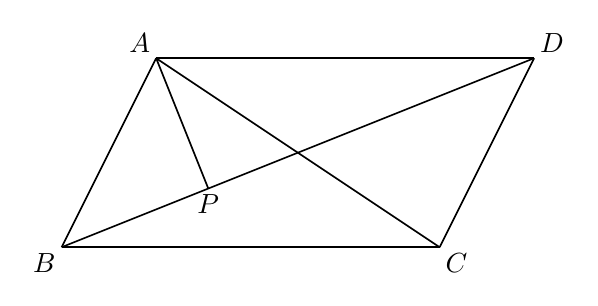
\begin{tikzpicture}[x=1cm,y=1cm,font=\normalsize,
 geometry edge/.style={solid,line width=.6pt},
 geometry mark/.style={solid,line width=.6pt},
 geometry label/.style={font=\normalsize,inner sep=2pt}]
\coordinate (A) at (0.000000000,2.400000000);
\coordinate (B) at (-1.200000000,0.000000000);
\coordinate (C) at (3.600000000,0.000000000);
\coordinate (D) at (4.800000000,2.400000000);
\coordinate (P) at (0.662068966,0.744827586);
\draw[geometry edge] (A)--(B);
\draw[geometry edge] (B)--(C);
\draw[geometry edge] (C)--(D);
\draw[geometry edge] (D)--(A);
\draw[geometry edge] (B)--(D);
\draw[geometry edge] (A)--(C);
\draw[geometry edge] (A)--(P);
\node[geometry label,above left] at (A) {$A$};
\node[geometry label,below left] at (B) {$B$};
\node[geometry label,below right] at (C) {$C$};
\node[geometry label,above right] at (D) {$D$};
\node[geometry label,below] at (P) {$P$};
\end{tikzpicture}
